\documentclass{llncs}
\usepackage{llncsdoc}

\usepackage{etex}
\usepackage[usenames,dvipsnames,svgnames,table]{xcolor}
\usepackage{listings}
\usepackage{pifont}
\usepackage{multirow}
\usepackage{amsmath}
\usepackage{amsfonts}
\usepackage{amssymb}
\usepackage{xspace}
\usepackage{graphicx}
\usepackage{lastpage}
\usepackage{paralist}
\usepackage{fancyhdr}
\usepackage{wrapfig}
\usepackage{balance}
\usepackage{tikz}
\usetikzlibrary{automata,shapes,arrows}
\usepackage{ctable} % for \specialrule command
\usepackage{pgfplots}
%\usepackage{amsthm}
\usepackage{dsfont}
\usepackage{colonequals}
\usepackage{enumitem}
\usepackage{wasysym}
\usepackage{mathtools}
\usepackage{listings}
%\usepackage{algorithm}
%\usepackage{algorithmic}
\usepackage{algpseudocode}
\usepackage{pifont}
\usepackage{stmaryrd}
\usepackage{comment}
\usepackage[hyphens]{url}
\usepackage{etoolbox}
\usepackage{pbox}
\usepackage{relsize}
\usepackage{csquotes}
\usepackage{scalerel}
\usepackage{setspace}
\usepackage[T1]{fontenc}
%\usepackage{euler}
\usepackage{manfnt}
\usepackage{tabularx}
\usepackage{hhline}
%\usepackage{titlesec}
\usepackage{enumitem}% http://ctan.org/pkg/enumitem
%\usepackage[showframe,pass]{geometry} %shows the margins of the page
\usepackage{wrapfig}

\newcommand{\den}[1]{\llbracket {#1} \rrbracket}

\newcommand{\alg}{\ensuremath{\mathrm{\Lambda}^*}\xspace}

\newcommand{\SFA}{\text{s-FA}\xspace}
\newcommand{\SFAs}{s-FAs\xspace}

%in-text enumeration
\newcommand{\rone}{(\emph{i})~}
\newcommand{\rtwo}{(\emph{ii})~}
\newcommand{\rthree}{(\emph{iii})~}
\newcommand{\rfour}{(\emph{iv})~}
\newcommand{\rfive}{(\emph{v})~}


\tikzset{->,auto,node distance=2.3cm,every node/.style={scale=0.7},baseline=(current bounding box.center)}

%%theorems if needed
%\theoremstyle{definition}
%\newtheorem{example}{Example}
%\AtEndEnvironment{example}{\null\hfill\qedsymbol}%
%\theoremstyle{plain}
%\newtheorem{theorem}{Theorem}
%\newtheorem{corollary}{Corollary}
%\newtheorem{lemma}{Lemma}
%\newtheorem{task}{Task}
%%\theoremstyle{definition}
%\newtheorem{definition}{Definition}
%%\AtEndEnvironment{definition}{\null\hfill\qedsymbol}%
\newcommand{\loris}[1]{{\color{blue}{L: #1}}}



\begin{document}

\title{Learning Symbolic Automata}
\author{Samuel Drews and Loris D'Antoni}
\institute{University of Wisconsin--Madison}

\maketitle
\begin{abstract}
Symbolic  automata allow transitions to carry predicates over
rich alphabet theories, such as linear arithmetic, and therefore extend
classic automata to operate over infinite alphabets, such as
the set of rational numbers. 
%Existing automata algorithms rely
%on the alphabet being finite, and generalizing them to the symbolic
%setting is not a trivial task.
In this paper, we study the foundational problem of learning symbolic automata.
We first present \alg,
a symbolic automata extension of Angluin's L$^*$
algorithm for learning regular languages.
Then, we define notions of learnability that are parametric in the alphabet theories
of the symbolic automata and show how these notions nicely compose.
Specifically, we show that if two alphabet theories are \emph{learnable},
then the theory accepting the Cartesian product or disjoint union of their alphabets is also learnable.
Using these properties, we show
how existing algorithms for learning automata over large alphabets nicely fall in our framework.
Finally, we implement our algorithm in an open-source library and evaluate it on existing automata learning benchmarks.
\end{abstract}

\section{Introduction}

Finite automata are a ubiquitous formalism that is simple enough to model many real-life systems and phenomena,
and they enjoy a large variety of theoretical properties:
automata are closed under Boolean operations,
have decidable emptiness and equivalence checking procedures, and
\emph{can be learned}~\cite{angluin87}.
This last problem on automata learning is the focus of this paper;
learning has been studied extensively for several variations of finite automata~\cite{Garcia08,Angluin15}
and has found many applications in program verification~\cite{Alur05} and
program synthesis~\cite{Yuan14}.

Unfortunately, finite automata have an inherent limitation: 
they can only operate over finite (and typically small) alphabets.
Symbolic finite  automata (\SFA) allow transitions to carry predicates over
rich alphabet theories, such as linear arithmetic, and therefore extend
classic automata to operate over infinite alphabets, such as
the set of rational numbers. 
Existing automata algorithms rely
on the alphabet being finite, and generalizing them to the symbolic
setting is not a trivial task. However, 
algorithms have been proposed for \SFA\ equivalence, for minimization, and for performing Boolean operations.
In this paper, we study the foundational problem of learning symbolic automata.

We start by
extending Angluin's L$^*$
algorithm~\cite{angluin87} for learning regular languages to symbolic automata.
L$^*$ iteratively updates a table of evidence, conjectures an automaton,
and then if that conjecture is not correct, repeats with new evidence.
However, at every step it must make a \emph{query} to an oracle
for each character in an alphabet;
thus it does not scale in practice on alphabets that are large
and cannot be run on those that are infinite.
Our algorithm, \alg, operates in a largely similar manner,
except that the queries are asked only for a small set of
representatives,
and then there is an additional stage after updating the table of evidence
during which the evidence is \emph{generalized} into symbolic predicates;
these predicates form the transitions for the symbolic automaton.

We then define notions of learnability that are parametric in the alphabet theory
of the symbolic automata and show that these notions compose.
For example, if two alphabet theories are \emph{learnable},
then the theory accepting the Cartesian product of their alphabets is also learnable.
We use these properties to show
how existing algorithms for learning automata over large alphabets nicely fall in our framework:
e.g., Maler and Mens present an ad hoc method for learning
automata over the alphabet
$\mathbb{Z} \times \mathbb{Z}$~\cite{mens15},
which we show is learnable because it is the Cartesian product of
of the alphabet $\mathbb{Z}$---which itself is learnable.

Finally, we implement our algorithm in an open-source symbolic automata library
and evaluate it on existing automata learning benchmarks
from~\cite{mens15}.
The implementation is  modular and only requires the programmer to provide
learnable Boolean algebras as input to the learner; the disjoint union and product algebras
are implemented as meta-algebras that can be instantiated arbitrarily.
Our implementation, despite its generality,
can learn the benchmarks appearing in~\cite{mens15}
using a similar number of equivalence and membership queries.

In summary, our contributions are:
\begin{itemize}
\vspace{-1mm}
\item An algorithm for learning Symbolic Finite Automata (\S~\ref{sec:learning}).
\item A notion of learnability parametric in the alphabet theory that composes over the 
		 Cartesian product and disjoint union of Boolean algebras (\S~\ref{sec:learnability}).
\item A modular implementation of our algorithm in an existing open-source library and an evaluation on existing benchmarks (\S~\ref{sec:implementation}).
\end{itemize}
%A full version of this paper that includes proofs is available at
%\url{http://tinyurl.com/hsfwcd6}.

\section{Preliminaries}

In symbolic automata, transitions carry predicates over a decidable Boolean algebra.
%\begin{definition}[Effective Boolean Algebra]
    An \emph{effective Boolean algebra} $\mathcal{A}$
    is a tuple $(\mathfrak{D}, \Psi, \den{\_}, \bot, \top, \vee, \wedge, \neg)$ where
    $\mathfrak{D}$ is a set of \emph{domain elements};
    $\Psi$ is a set of \emph{predicates} closed under the Boolean connectives, with $\bot, \top \in \Psi$;
    $\den{\_} : \Psi \rightarrow 2^\mathfrak{D}$
    is a \emph{denotation function} such that
    \rone $\den{\bot} = \emptyset$,
    \rtwo $\den{\top} = \mathfrak{D}$,
    and \rthree for all $\varphi, \psi \in \Psi$,
        $\den{\varphi \vee \psi} = \den{\varphi} \cup \den{\psi}$,
        $\den{\varphi \wedge \psi} = \den{\varphi} \cap \den{\psi}$,
        and $\den{\neg \varphi} = \mathfrak{D} \setminus \den{\varphi}$.
%\end{definition}

%Since $\Psi$ is closed with respect to $\vee$, $\wedge$, and $\neg$,
%we can \emph{generate} $\Psi$ from an initial set $\Psi_0$ as follows:
%for all $i > 0$,
%\begin{align*}
%    \Psi_{i+1} = \Psi_i &\cup \{\neg \varphi \mid \varphi \in \Psi_i\}
%        \cup \{\varphi_1 \vee \varphi_2 \mid \varphi_1, \varphi_2 \in \Psi_i\} 
%        \cup \{\varphi_1 \wedge \varphi_2 \mid \varphi_1, \varphi_2 \in \Psi_i\}
%\end{align*}
%And finally, $\Psi = \bigcup_i \Psi_i$ for all $i \geq 0$.
%
%Consider the following examples of Boolean algebras:

\begin{example}[Equality Algebra]
    %Let $c$ be a fixed variable.
    The \emph{equality algebra} for an arbitrary set $\mathfrak{D}$
    has predicates formed from Boolean combinations of
    formulas of the form $\lambda c \ldotp c = a$ where $a \in \mathfrak{D}$.
    Formally, $\Psi$ is generated from the Boolean closure of
    $\Psi_0 = \{\varphi_a \mid a \in \mathfrak{D}\} \cup \{\bot, \top\}$
    where for all $a \in \mathfrak{D}$, $\den{\varphi_a} = \{a\}$.
    Example predicates in this algebra include the predicates
    %$c = 5 \vee c = 10$ and $\neg(c = 0)$.
    $\lambda c \ldotp c = 5 \vee c = 10$ and $\lambda c \ldotp \neg(c = 0)$.
\end{example}

\begin{example}[Interval Algebra]
\label{ex:interval}
    The finite union of left-closed right-open intervals over 
    non-negative integers (i.e. $\mathbb{N}$) also forms a Boolean algebra:
    take the Boolean closure of
    $\Psi_0 = \{\varphi_{ij} \mid i,j \in \mathbb{N} \land i < j\} \cup \{\bot, \top\}$
    where $\den{\varphi_{ij}} = [i, j)$.
    Example predicates in this algebra include those
    (written as their denotation) of the form
    $[0,5) \cup [10,15)$ or $[50,\infty)$.
\end{example}

%Now we are ready to present the formalism of symbolic finite automata.

\begin{definition}[Symbolic Finite Automata]
A \emph{symbolic finite automaton} (\SFA) $M$
is a tuple $(\mathcal{A}, Q, q_\text{init}, F, \Delta)$ where
$\mathcal{A}$ is an effective Boolean algebra, called the \emph{alphabet};
$Q$ is a finite set of states;
$q_\text{init} \in Q$ is the \emph{initial state};
$F \subseteq Q$ is the set of \emph{final states};
and $\Delta \subseteq Q \times \Psi_\mathcal{A} \times Q$
is the \emph{transition relation} consisting of
a finite set of \emph{moves} or \emph{transitions}.
\end{definition}
%
\emph{Characters} are elements of $\mathfrak{D}_\mathcal{A}$,
and \emph{words} are finite sequences of characters,
or elements of $\mathfrak{D}_\mathcal{A}^*$.
The empty word of length 0 is denoted by $\epsilon$.
A move $\rho = (q_1, \varphi, q_2) \in \Delta$,
also denoted $q_1 \xrightarrow{\varphi} q_2$,
is a transition from the \emph{source} state $q_1$
to the \emph{target} state $q_2$,
where $\varphi$ is the \emph{guard} or \emph{predicate} of the move.
A move is \emph{feasible} if its guard is satisfiable.
%
For a character $a \in \mathfrak{D}_\mathcal{A}$, 
an \emph{a-move} of $M$, denoted $q_1 \xrightarrow{a} q_2$
is a move $q_1 \xrightarrow{\varphi} q_2$
such that $a \in \den{\varphi}$.

An \SFA\ $M$ is \emph{deterministic} if, for all transitions
$(q, \varphi_1, q_1), (q, \varphi_2, q_2) \in \Delta$,
$q_1 \neq q_2 \rightarrow \den{\varphi_1 \wedge \varphi_2} = \emptyset$;
i.e., for each state $q$ and character $a$ there is at most one $a$-move
out of $q$.
An \SFA\ $M$ is \emph{complete} if, for all $q \in Q$,
$\bigvee_{(q, \varphi_i, q_i) \in \Delta} \varphi_i = \top$;
i.e., for each state $q$ and character $a$ there exists an $a$-move
out of $q$.
Throughout the paper we assume all \SFAs\ are
deterministic and complete, since
determinization and completion are always possible~\cite{dantoni14}.
An example \SFA\ is $\mathbf{M_{11}}$ in Figure~\ref{fig:example}.
This {\SFA} has 4 states and it operates over the interval algebra from Example~\ref{ex:interval}.

Given an \SFA\ $M = (\mathcal{A}, Q, q_\text{init}, F, \Delta)$
and a state $q \in Q$, 
we say a word $w = a_1 a_2 \ldots a_k$ is \emph{accepted at state $q$}
if, for $1 \leq i \leq k$, there exist moves $q_{i-1} \xrightarrow{a_i} q_i$
such that $q_0 = q$ and $q_k \in F$.
We refer to the set of words accepted at $q$ as the
\emph{language accepted at $q$}, denoted as $\mathcal{L}_q(M)$;
the \emph{language accepted by $M$} is
$\mathcal{L}(M) = \mathcal{L}_{q_\text{init}}(M)$.
%
The \SFA\ $\mathbf{M_{11}}$ in Figure~\ref{fig:example}
accepts, among others, words consisting only of numbers accepted by the predicate $[0,51)\cup[101,\infty)$
and rejects, among others, the word  $51,25$.

\section{Learning Algorithm}
\label{sec:learning}

Here we present our algorithm, \alg,
for learning symbolic automata.
The premise is that the automaton to be learned,
called the \emph{target},
is hidden in a black box,
so knowledge of it comes from some \emph{oracle}
that admits two kinds of queries:
\emph{membership queries} that ask
whether a word is in the language of the target, and
\emph{equivalence queries} that ask
whether a conjectured automaton is equivalent
to the target---if not, a 
counterexample is provided.
\alg, which builds upon L$^*$~\cite{angluin87},
maintains an \emph{observation table}
that comprises its knowledge about the target.
The observation table is used to build the intermediary guesses of the target automaton
and, eventually, the final automaton.
It is assumed that the learner knows
both the alphabet and the Boolean algebra in question. 
%We assume the learner knows the Boolean algebra over which that automaton operates.

\subsection{Observation Table}

The observation table consists of
rows of prefixes and columns of suffixes.
Each entry determines whether the target automaton
accepts the word formed by concatenating
the prefix and suffix.
Intuitively, prefixes
provide knowledge about words that
lead to states,
and suffixes help differentiate those states.

\begin{definition}[Observation Table]
    An \emph{observation table} $T$ for an \SFA\ $M$
    is a tuple $(\Sigma, S, R, E, f)$ where
    $\Sigma$ is a potentially infinite set called the \emph{alphabet};
    $S,R,E \subset \Sigma^*$ are finite subsets of words:
        $S$ is called the set of \emph{prefixes}, 
        $R$ is called the \emph{boundary},
        and $E$ is called the set of \emph{suffixes};
    $f : (S \cup R) \cdot E \rightarrow \{0,1\}$
        is a \emph{classification function}\footnote{We
        also use $\{-,+\}$ to denote the range of $f$.}
        such that
        for a word $w \cdot e \in (S \cup R) \cdot E$,
        $f(w \cdot e) = 1$ if $w \cdot e \in \mathcal{L}(M)$, and
        $f(w \cdot e) = 0$ if $w \cdot e \not\in \mathcal{L}(M)$.%
        \footnote{We use $\cdot$ to denote both the concatenation
        of strings and its lifting to sets of strings,
        as is standard.}
    Additionally, %the following properties hold:
    \rone $S$ and $R$ are disjoint,
    \rtwo $S \cup R$ is prefix-closed and $\epsilon \in S$,
    \rthree for all $s \in S$, there exists a character $a \in \Sigma$ such that $s \cdot a \in R$,
    and \rfour $\epsilon \in E$.
\end{definition}
%
Table $\mathbf{T_1}$ in Figure~\ref{fig:example} is an example observation table:
The rows begin with elements of $S \cup R$,
where the elements in $S$ are shown above the horizontal divider
and the elements in $R$ below,
and the columns begin with elements of $E$.

The observation table induces the construction of an automaton.
For intuition,
each $s \in S$ corresponds to a state $q$ 
such that $s$ is a string of moves
from $q_\text{init}$ to $q$.
The boundary $R$ gives information about the 
transitions between states.
The states are differentiated by the 
strings in $E$ and the classification function $f$,
as if there exist $s_1, s_2 \in S$ and $e \in E$
such that $f(s_1 \cdot e) \neq f(s_2 \cdot e)$,
then $s_1$ and $s_2$ \emph{behave} differently 
and must lead to different states.
We use the notation $\textit{row}(w)$ for $w \in S \cup R$
to denote the vector indexed by $e \in E$ of $f(w \cdot e)$.

\alg\ manipulates the observation table and eventually
conjectures an \SFA.  For this to happen, the table must first satisfy certain properties---we
call such a table \emph{cohesive}---that
are established through membership queries to the oracle.
The cohesive observation table is used
to construct an intermediary automaton
that is ultimately used to produce a conjectured \SFA.
An observation table is \emph{closed} 
if for each $r \in R$ there exists $s \in S$
such that $\textit{row}(s) = \textit{row}(r)$;
in other words, each element in the boundary
corresponds to a state.
%
An observation table is \emph{reduced}
if for all $s_1, s_2 \in S$,
$\textit{row}(s_1) \neq \textit{row}(s_2)$,
meaning each state is uniquely characterized by $f$ and $E$.
%
An observation table is \emph{consistent}
if for all $w_1, w_2 \in S \cup R$,
if $a \in \Sigma^*$ and $w_1 \cdot a, w_2 \cdot a \in S \cup R$
and $\textit{row}(w_1) = \textit{row}(w_2)$, then
$\textit{row}(w_1 \cdot a) = \textit{row}(w_2 \cdot a)$.
%
A table being consistent means that if the words $w_1$ and $w_2$
are equivalent according to $f$ and $E$,
then $w_1 \cdot a$ and $w_2 \cdot a$ ought to be
equivalent as well, and thus
there is no evidence to the contrary.\footnote{We
use $a \in \Sigma^*$ for the definition
of \emph{consistent}, but since the table
is prefix-closed by definition,
it is equivalent to consider
only single-characters $a \in \Sigma$.}
%
An observation table is \emph{evidence-closed}
if for all $e \in E$ and $s \in S$,
$s \cdot e \in S \cup R$.
%
An observation table is \emph{cohesive}
if it is closed, reduced, consistent, and evidence-closed.

Consider, for example, the observation tables in Figure~\ref{fig:example}.
$\mathbf{T_2}$  is not closed, since $\textit{row}(51) = -$
and there is no $s \in S$ with $\textit{row}(s) = -$.
Table $\mathbf{T_5}$ is not
consistent because $\textit{row}(51) = - = \textit{row}(51,0)$,
but $\textit{row}(51\cdot0) = - \neq + = \textit{row}(51,0\cdot0)$.
Table $\mathbf{T_{11}}$ is closed, reduced, consistent, and evidence-closed.

If an observation table is cohesive,
then it admits the construction of an \emph{evidence automaton}
that classifies words $w \in \Sigma^*$
equivalently to the observation table's classification function $f$.

\begin{definition}[Evidence Automaton]
    An evidence automaton is a tuple
    $(\Sigma, Q, q_\text{init}, F, \Delta)$ where
    $\Sigma$ is a set;
    $Q$ is a finite set of states;
    $q_\text{init} \in Q$ is the \emph{initial state};
    $F \subseteq Q$ is the set of \emph{final states};
    $\Delta \subseteq Q \times \Sigma \times Q$ is the \emph{transition relation}.
\end{definition}
A move $\rho = (q_1, a, q_2)$,
also denoted $q_1 \xrightarrow{a} q_2$,
is a transition from $q_1$ to $q_2$ using the character $a$.  
A word $w = a_1 a_2 \ldots a_k$ is \emph{accepted at state $q$}
if for $1 \leq i \leq k$ there exist moves
$q_{i-1} \xrightarrow{a_i} q_i$ such that $q_0 = q$ and $q_k \in F$.
Conversely, if that $q_k \not \in F$, 
then $w$ is \emph{not} accepted at $q$.
If there is no path through the automaton for $w$,
then the acceptance is undefined.
An evidence automaton differs from an \SFA
in that transitions carry characters in $\Sigma$ instead of predicates
in a Boolean algebra over the domain $\Sigma$.
Additionally, the evidence automaton can be deliberately sparse:
it is not \emph{complete}, and we avoid 
the notion that a state $q$ does not accept a character $a$
if there is no $q'$ such that $(q, a, q') \in \Delta$---as
stated above, such
a case simply indicates the behavior of $a$ at $q$ is undefined.

Given a cohesive observation table
$T = (\Sigma, S, R, E, f)$, we build an evidence automaton
$A = (\Sigma, Q, q_\text{init}, F, \Delta)$
%over that same alphabet
as follows:
for each $s \in S$, we introduce a state $q_s \in Q$. %, and
$q_\text{init}$ is assigned to $q_\epsilon$.
The final state set $F$ contains   all $q_s$ such that $s \in S$ and $f(s) = 1$.
%
Since the observation table is closed and reduced,
there exists a function $g : S \cup R \rightarrow S$
such that $g(w) = s$ if and only if $row(w) = row(s)$.
This function allows us to define the transition relation of $A$:
if $w \cdot a \in S \cup R$ for $w \in \Sigma^*$ and $a \in \Sigma$, then 
$(q_{g(w)}, a, q_{g(w \cdot a)}) \in \Delta$.
%
In Figure~\ref{fig:example}, the automaton $\mathbf{M_{1}^e}$ (resp $\mathbf{M_{11}^e}$) is the evidence automaton 
corresponding to cohesive table $\mathbf{T_{1}}$ (resp. $\mathbf{T_{11}}$).


\begin{lemma}[Evidence compatibility]\label{thm:evid}
    Given a cohesive observation table $T = (\Sigma, S, R, E, f)$,
    if $M_\text{evid} = (\Sigma, Q, q_\text{init}, F, \Delta)$ 
    is the evidence automaton construction of $T$,
    then for all $w \cdot e \in (S \cup R) \cdot E$,
    if $f(w \cdot e) = 1$ then $M_\text{evid}$ accepts $w \cdot e$, and
    if $f(w \cdot e) = 0$ then $M_\text{evid}$ does not accept $w \cdot e$.
\end{lemma}

\subsection{Separating Predicates}

Given an evidence automaton with an alphabet $\Sigma$,
we require two pieces to build an \SFA:
\rone a Boolean algebra $\mathcal{A}$ with $\mathfrak{D}_\mathcal{A} = \Sigma$,
and \rtwo a partitioning function $P$ for $\mathcal{A}$, which we define below.
%
This latter component,
the partitioning function,
is the key insight to \alg's
generalization of L$^*$.

\begin{definition}[Partitioning function]
    A \emph{partitioning function} for a Boolean algebra
    $\mathcal{A} = (\mathfrak{D}, \Psi, \den{\_}, \bot, \top, \vee, \wedge, \neg)$
    is a function $P : (2^\mathfrak{D})^* \rightarrow \Psi^*$
    that takes as input a list $L_\mathfrak{D} = \ell_1 \ldots \ell_k$
    of disjoint sets of elements in $\mathfrak{D}$,
    and returns a parallel list $L_\Psi = \varphi_1 \ldots \varphi_k$ of predicates in $\Psi$ such that
    \begin{itemize}
        \item $\bigvee_{\varphi_i \in L_\Psi} \varphi_i = \top$
        \item $\varphi_i \wedge \varphi_j = \bot$ for all $\varphi_i, \varphi_j \in L_\Psi$ with $i \neq j$
        \item for each $\ell_i \in L_\mathfrak{D}$ corresponding to $\varphi_i \in L_\Psi$,
            all $a \in \ell_i$ are such that $a \in \den{\varphi_i}$.
    \end{itemize}
\end{definition}

\begin{example}[Equality Algebra Separating Predicates]
    We can construct a partitioning function for the equality algebra:
    given a list
    $L_\mathfrak{D} = \ell_1 \ldots \ell_k$
    we construct a list $L_\Psi = \varphi_1 \ldots \varphi_k$
    where each $\varphi_i$ has $\den{\varphi_i} = \ell_i$.
    We choose a $j$ with maximal $|\ell_j|$
    and update $\varphi_j \gets \varphi_j \vee \bigwedge_{1 \leq i \leq k} \neg \varphi_i$.
    In the concrete case of $\mathfrak{D} = \mathbb{Z}$ 
    and $L_\mathfrak{D} = [\{2\}, \{3\}, \emptyset, \{0, 5\}]$,
    the partitioning function would produce (after simplification)
    %$L_\Psi = [a = 2, a = 3, \bot, a \neq 2 \wedge a \neq 3]$.
    $L_\Psi = [\lambda a \ldotp a = 2, \lambda a \ldotp a = 3, \bot, \lambda a \ldotp a \neq 2 \wedge a \neq 3]$.
\end{example}

At a high level, as long as the \SFA is consistent with the evidence automaton,
it will be consistent with the observation table.
The words in the remainder of $\Sigma^*$---for which 
the evidence automaton has unspecified classification---can be
assigned to paths in a largely arbitrary manner.
The partitioning function handles generalizing the concrete evidence
by creating \emph{separating predicates}, 
in effect specifying the behavior for the remaining words.
Ideally, this generalization allows an automaton to be learned
with a relatively small observation table,
even if the alphabet is large---or even infinite.

Given an evidence automaton $A = (\Sigma, Q, q_\text{init}, F, \Delta)$,
a Boolean algebra $\mathcal{A}$ with domain $\Sigma$, and an 
appropriate partitioning function $P$,
we build an \SFA $M = (\mathcal{A}, Q, q_\text{init}, F, \Delta_M)$
using that Boolean algebra and that exact configuration of states.
All that remains is the construction of the transition relation $\Delta_M$.

For each  $q \in Q$, we perform the following.
We gather all evidence transitions out of $q$
into a set $\Delta_q = \{(q, a, q') \in \Delta\}$
and construct a list $L_\Sigma$ indexed over the states $q_i \in Q$,
where each set in $L_\Sigma$ is $\ell_i = \{a \mid (q, a, q_i) \in \Delta_q\}$.
We apply the partitioning function to 
get a list of separating predicates
$L_{\Psi_\mathcal{A}} = P(L_\Sigma)$
which is also indexed over $q_i \in Q$,
and add $(q, \varphi_i, q_i)$ to $\Delta_M$ for each $\varphi_i \in L_{\Psi_\mathcal{A}}$.

\begin{lemma}[\SFA evidence compatibility]\label{thm:evid2}
    Given a cohesive observation table $T = (\Sigma, S, R, E, F)$,
    if $M_\text{evid} = (\Sigma, Q, q_\text{init}, F, \Delta)$
    is the evidence automaton construction of $T$, and
    $M = (\mathcal{A}, Q, q_\text{init}, F, \Delta)$
    is produced from $M_\text{evid}$ using a partitioning function,
    then for all $w \cdot e \in (S \cup R) \cdot E$,
    if $f(w \cdot e) = 1$ then $w \cdot e \in \mathcal{L}(M)$, and
    if $f(w \cdot e) = 0$ then $w \cdot e \not \in \mathcal{L}(M)$.
\end{lemma}

An example observation table, its corresponding evidence automaton, 
and a resultant \SFA are shown in the last row of Figure~\ref{fig:example}.



\subsection{Algorithm Description}

We now present a description of \alg and an example execution.
The algorithm begins by initializing an observation table
with $S = \{\epsilon\}$, $R = \{a\}$ for an arbitrary $a \in \Sigma$,
and $E = \{\epsilon\}$.
$f$ is initially undefined.
The knowledge of the table
is grown using the operations
\emph{fill}, \emph{close}, \emph{evidence-close}, and \emph{make-consistent}.

The operation \emph{fill} asks a membership query
for all $w \cdot e \in (S \cup R) \cdot E$ for which
$f$ is undefined and then adds those results to $f$;
in this way, it ensures $f$ is defined over the 
entire domain of the observation table.

The operation \emph{close} checks for
the existence of an $r \in R$ such that
for all $s \in S$, $\textit{row}(r) \neq \textit{row}(s)$.
Such an $r$ is moved from $R$ to $S$,
and $r \cdot a$ is added to $R$
for some arbitrary $a \in \Sigma$.

The operation \emph{evidence-close} ensures
for all $e \in E$ and $s \in S$ that
$s \cdot e \in S \cup R$
by adding to $R$ all $s \cdot e$
that are not.
It also adds to $R$ any necessary prefixes
so that $S \cup R$ is prefix-closed.

The operation \emph{make-consistent} operates as follows:
if there exist $w_1, w_2 \in S \cup R$
and $w_1 \cdot a, w_2 \cdot a \in S \cup R$
for some $a \in \Sigma$
such that $\textit{row}(w_1) = \textit{row}(w_2)$
but $\textit{row}(w_1 \cdot a) \neq \textit{row}(w_2 \cdot a)$,
then $w_1$ and $w_2$ actually lead to different states;
using the $e \in E$ such that $f(w_1 \cdot a \cdot e) \neq f(w_2 \cdot a \cdot e)$,
it is clear $a \cdot e$ thus differentiates those states.
Accordingly, $a \cdot e$ is added to $E$.
Additionally, we then add
$(\{u_2 \cdot b \mid u_1 \cdot b \in S \cup R\} \cup \{u_1 \cdot b \mid u_2 \cdot b \in S \cup R\}) \setminus S$
to $R$ for all pairs $u_1, u_2 \in S \cup R$ such that before adding $e$ to $E$,
$\textit{row}(u_1) = \textit{row}(u_2)$,
but $f(u_1 \cdot e) \neq f(u_2 \cdot e)$
(this includes the pair $w_1, w_2$).
This operation \emph{distributes} the old evidence leading
    out of the amalgamated state between the newly differentiated states,
simplifying the constructions in Section~\ref{sec:learnability}.

Upon receiving a counterexample $c \in \Sigma^*$ from 
an equivalence query sent to the oracle,
all prefixes of $c$ are added to $R$
(except those already present in $S$).
There are two cases for a counterexample:
one of the predicates in the \SFA needs refinement,
which is facilitated by adding those new words to the table,
or a new state must exist in the automaton,
which is handled by \emph{make-consistent}.

\algrenewcommand\algorithmicindent{1.0em}
\newcommand\NoThen{\renewcommand\algorithmicthen{}}
\algtext*{EndWhile}% Remove "end while" text
\algtext*{EndIf}
\algtext*{EndProcedure}
\begin{figure}[!t]
%\begin{minipage}{0.5\textwidth}
%%\begin{algorithm}[t]
%%    \caption{Learning algorithm}
%    \scriptsize
%    \begin{algorithmic}
%       \Procedure{\alg}{$M$}
%        \State initialize table $T$
%        \Repeat
%        \While{$T$ is not cohesive}
%        \State \emph{make-consistent} $T$
%        \State \emph{evidence-close} $T$
%        \State \emph{close} $T$
%        \EndWhile
%        \State build evidence automaton $M_\textit{evid}$ from $T$
%        \State build \SFA $M$ from $M_\textit{evid}$
%        \If{$M$ $\neq$ target automaton} 
%        \State process counterexample
%        \EndIf
%        \Until{$M$ $=$ target automaton}
%        \EndProcedure
%    \end{algorithmic}
%%\end{algorithm}
%\end{minipage}
%\begin{minipage}{0.5\textwidth}
\centering
\tikzstyle{block} = [rectangle, draw, text width=6em, text centered, rounded corners, minimum height =4em]
\begin{tikzpicture}[->,>=stealth',auto,node distance = 3.5cm]
    \node [draw=none] (0) {};
    \node [block] (1) [right of=0] {is table cohesive?};
    \node [block] (2) [right of=1] {build evidence automaton};
    \node [block] (3) [right of=2,xshift=1.5cm] {build \SFA; is equivalent?};
    \node [block] (4) [right of=3] {done};
    \path 
    (0) edge node[align=center] {initialize\\table} (1)
    (1) edge node {yes} (2)
    (1) edge [loop above] node[align=center] {no:\\membership queries} (1)
    (2) edge node[align=center] {partitioning\\function} (3)
    (3) edge node {yes} (4)
    (3) edge [bend left] node[align=center] {no:\\add counterexample to table} (1)
    ;
\end{tikzpicture}
%\end{minipage}
%\caption{Pseudocode of the learning algorithm \alg (left) and its overview (right).\label{alg:learn}}
\caption{Overview of the learning algorithm \alg.\label{alg:learn}}
\end{figure}

Figure~\ref{alg:learn} shows an overview of the learning algorithm:
after the table is initialized,
the operations \emph{make-consistent},
\emph{evidence-close}, and \emph{close}
are applied until the table is cohesive.\footnote{
It is an invariant of the initialization of the table
and of the operations applied to it
that the observation table is always reduced.}
(\emph{Fill} is applied throughout whenever
a change is made to the table.)
An \SFA $M$ is then conjectured from the table,
and an equivalence query is performed:
if $M$ is equivalent to the target automaton,
then the algorithm terminates.
Otherwise, a counterexample is produced and processed,
and the procedure repeats.

\alg can be thought of as a lazily-evaluated version
of L$^*$ with the additional generalization step,
and therefore it maintains the property of L$^*$
that the learned automaton has a minimal
number of states.

\begin{theorem}[\alg minimality]\label{thm:min}
    When \alg terminates it returns a minimal \SFA.
\end{theorem}

\begin{figure}
    \begin{tabular}{c}
        \begingroup
\scriptsize
\begin{tabular}{r | c}
    $\mathbf{T_1}$ & $\epsilon$ \\ \hline
    $\epsilon$ & + \\ \hline
    0 & +
\end{tabular}
\endgroup

        \begin{tabular}{l}
            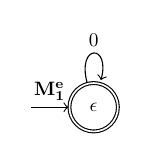
\begin{tikzpicture}
    \node[state,accepting] (1) {$\epsilon$};
    \draw[<-] (1) -- node[above] {$\mathbf{M_1^e}$} ++(-.8cm,0);
    \path
    (1) edge [loop above] node {0} (1)
    ;
\end{tikzpicture}
 \\[.75cm]
            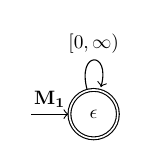
\begin{tikzpicture}
    \node[state,accepting] (1) {$\epsilon$};
    \draw[<-] (1) -- node[above] {$\mathbf{M_1}$} ++(-.8cm,0);
    \path
    (1) edge [loop above] node {$[0,\infty)$} (1)
    ;
\end{tikzpicture}

        \end{tabular}
        $\xRightarrow{51~-}$
        \begingroup
\scriptsize
\begin{tabular}{r | c}
    $\mathbf{T_2}$ & $\epsilon$ \\ \hline
    $\epsilon$ & + \\ \hline
    0 & + \\
    51 & -
\end{tabular}
\endgroup
 
        $\xRightarrow{\text{close}}$
        \begingroup
\scriptsize
\begin{tabular}{r | c}
    $\mathbf{T_3}$ & $\epsilon$ \\ \hline
    $\epsilon$ & + \\
    51 & - \\ \hline
    0 & + \\
    51,0 & -
\end{tabular}
\endgroup

        \begin{tabular}{l}
            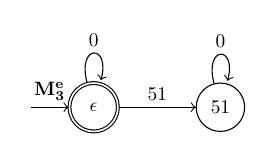
\begin{tikzpicture}
    \node[state,accepting] (1) {$\epsilon$};
    \draw[<-] (1) -- node[above] {$\mathbf{M_3^e}$} ++(-.8cm,0);
    \node[state] (2) [right of=1] {51};
    \path
    (1) edge [loop above] node {0} (1)
    (1) edge node {51} (2)
    (2) edge [loop above] node {0} (2)
    ;
\end{tikzpicture}
 \\[.75cm]
            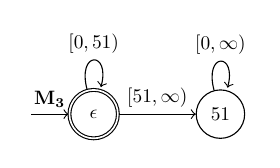
\begin{tikzpicture}
    \node[state,accepting] (1) {$\epsilon$};
    \draw[<-] (1) -- node[above] {$\mathbf{M_3}$} ++(-.8cm,0);
    \node[state] (2) [right of=1] {51};
    \path
    (1) edge [loop above] node {$[0,51)$} (1)
    (1) edge node {$[51,\infty)$} (2)
    (2) edge [loop above] node {$[0,\infty)$} (2)
    ;
\end{tikzpicture}

        \end{tabular} 
        $\xRightarrow{101~+}$        
        \\[1.6cm]
        %
        \begingroup
\scriptsize
\begin{tabular}{r | c}
    $\mathbf{T_4}$ & $\epsilon$ \\ \hline
    $\epsilon$ & + \\
    51 & - \\ \hline
    0 & + \\
    51,0 & - \\
    101 & +
\end{tabular}
\endgroup

        \begin{tabular}{r}
            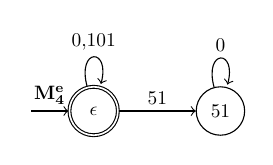
\begin{tikzpicture}
    \node[state,accepting] (1) {$\epsilon$};
    \draw[<-] (1) -- node[above] {$\mathbf{M_4^e}$} ++(-.8cm,0);
    \node[state] (2) [right of=1] {51};
    \path
    (1) edge [loop above] node {0,101} (1)
    (1) edge node {51} (2)
    (2) edge [loop above] node {0} (2)
    ;
\end{tikzpicture}
 \\[.75cm]
            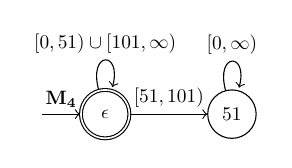
\begin{tikzpicture}
    \node[state,accepting] (1) {$\epsilon$};
    \draw[<-] (1) -- node[above] {$\mathbf{M_4}$} ++(-.8cm,0);
    \node[state] (2) [right of=1] {51};
    \path
    (1) edge [loop above] node {$[0,51) \cup [101,\infty)$} (1)
    (1) edge node {$[51,101)$} (2)
    (2) edge [loop above] node {$[0,\infty)$} (2)
    ;
\end{tikzpicture}

        \end{tabular}
        $\xRightarrow{51,0,0~+}$
        \begingroup
\scriptsize
\begin{tabular}{r | c}
    $\mathbf{T_5}$ & $\epsilon$ \\ \hline
    $\epsilon$ & + \\
    51 & - \\ \hline
    0 & + \\
    51,0 & - \\
    101 & + \\
    51,0,0 & +
\end{tabular}
\endgroup

        $\xRightarrow{
        \begin{scriptsize}                                     
        \begin{array}{c}
         \text{make}\\
         \text{consistent}
		\end{array}
		\end{scriptsize}    
        }$
        \begingroup
\scriptsize
\begin{tabular}{r | c c}
    $\mathbf{T_6}$ & $\epsilon$ & 0\\ \hline
    $\epsilon$ & + & + \\
    51 & - & - \\ \hline
    0 & + & + \\
    51,0 & - & + \\
    101 & + & + \\
    51,0,0 & + & +
\end{tabular}
\endgroup
 
        $\xRightarrow{\text{close}}$             
        \\[1.6cm]
        %
        \hspace{-7mm}
        \begingroup
\scriptsize
\begin{tabular}{r | c c}
    $\mathbf{T_7}$ & $\epsilon$ & 0\\ \hline
    $\epsilon$ & + & + \\
    51 & - & - \\
    51,0 & - & + \\ \hline
    0 & + & + \\
    101 & + & + \\
    51,0,0 & + & +
\end{tabular}
\endgroup
\hspace{-1mm}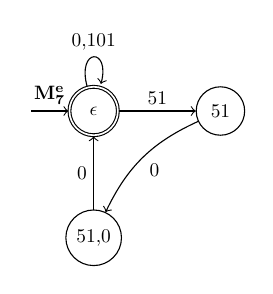
\begin{tikzpicture}
    \node[state,accepting] (1) {$\epsilon$};
    \draw[<-] (1) -- node[above] {$\mathbf{M_7^e}$} ++(-.8cm,0);
    \node[state] (2) [right of=1] {51};
    \node[state] (3) [below of=1] {51,0};
    \path
    (1) edge [loop above] node {0,101} (1)
    (1) edge node {51} (2)
    (2) edge [bend right=20] node {0} (3)
    (3) edge node {0} (1)
    ;
\end{tikzpicture}
\hspace{-2mm}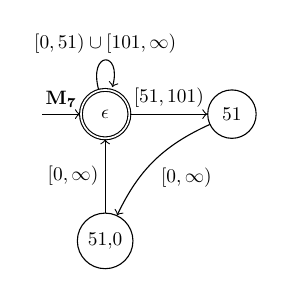
\begin{tikzpicture}
    \node[state,accepting] (1) {$\epsilon$};
    \draw[<-] (1) -- node[above] {$\mathbf{M_7}$} ++(-.8cm,0);
    \node[state] (2) [right of=1] {51};
    \node[state] (3) [below of=1] {51,0};
    \path
    (1) edge [loop above] node {$[0,51) \cup [101,\infty)$} (1)
    (1) edge node {$[51,101)$} (2)
    (2) edge [bend right=20] node {$[0,\infty)$} (3)
    (3) edge node {$[0,\infty)$} (1)
    ;
\end{tikzpicture}

        $\xRightarrow{
        \begin{scriptsize}                                     
        \begin{tiny}
        \begin{array}{c}
         51,21,0\\
         -
		\end{array}
        \end{tiny}		
		\end{scriptsize}    
        }$
        \begingroup
\scriptsize
\begin{tabular}{r | c c}
    $\mathbf{T_8}$ & $\epsilon$ & 0\\ \hline
    $\epsilon$ & + & + \\
    51 & - & - \\
    51,0 & - & + \\ \hline
    0 & + & + \\
    101 & + & + \\
    51,0,0 & + & + \\
    51,21 & - & - \\
    51,21,0 & - & -
\end{tabular}
\endgroup

        $\xRightarrow{
        \begin{scriptsize}                                     
        \begin{array}{c}
         \text{mk}\\
         \text{cons.}
		\end{array}
		\end{scriptsize}    
        }$
        \begingroup
\scriptsize
\begin{tabular}{r | c c c}
    $\mathbf{T_9}$ & $\epsilon$ & 0 & 0,0\\ \hline
    $\epsilon$ & + & + & + \\
    51 & - & - & + \\
    51,0 & - & + & + \\ \hline
    0 & + & + & + \\
    101 & + & + & + \\
    51,0,0 & + & + & + \\
    51,21 & - & - & - \\
    51,21,0 & - & - & - \\
    0,0 & + & + & + \\
    51,0,0,0 & + & + & +
\end{tabular}
\endgroup
\\[1.6cm]
        %         
        $\xRightarrow{\text{close}}$
        \begingroup
\scriptsize
\begin{tabular}{r | c c c}
    $\mathbf{T_{10}}$ & $\epsilon$ & 0 & 0,0\\ \hline
    $\epsilon$ & + & + & + \\
    51 & - & - & + \\
    51,0 & - & + & + \\
    51,21 & - & - & - \\ \hline
    0 & + & + & + \\
    101 & + & + & + \\
    51,0,0 & + & + & + \\
    51,21,0 & - & - & - \\
    0,0 & + & + & + \\
    51,0,0,0 & + & + & + \\
    51,21,0,0 & - & - & -
\end{tabular}
\endgroup
 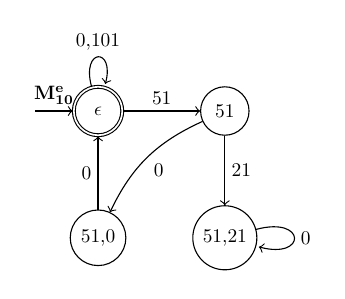
\begin{tikzpicture}
    \node[state,accepting] (1) {$\epsilon$};
    \draw[<-] (1) -- node[above] {$\mathbf{M_{10}^e}$} ++(-.8cm,0);
    \node[state] (2) [right of=1] {51};
    \node[state] (3) [below of=1] {51,0};
    \node[state] (4) [below of=2] {51,21};
    \path
    (1) edge [loop above] node {0,101} (1)
    (1) edge node {51} (2)
    (2) edge [bend right=20] node {0} (3)
    (2) edge node {21} (4)
    (3) edge node {0} (1)
    (4) edge [loop right] node {0} (4)
    ;
\end{tikzpicture}
\hspace{-1mm}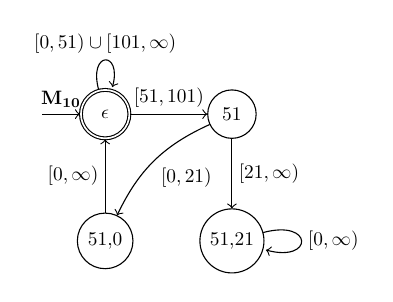
\begin{tikzpicture}
    \node[state,accepting] (1) {$\epsilon$};
    \draw[<-] (1) -- node[above] {$\mathbf{M_{10}}$} ++(-.8cm,0);
    \node[state] (2) [right of=1] {51};
    \node[state] (3) [below of=1] {51,0};
    \node[state] (4) [below of=2] {51,21};
    \path
    (1) edge [loop above] node {$[0,51) \cup [101,\infty)$} (1)
    (1) edge node {$[51,101)$} (2)
    (2) edge [bend right=20] node {$[0,21)$} (3)
    (2) edge node {$[21,\infty)$} (4)
    (3) edge node {$[0,\infty)$} (1)
    (4) edge [loop right] node {$[0,\infty)$} (4)
    ;
\end{tikzpicture}
 \\[2cm]
        %
        $\xRightarrow{51,0,21~-}$
        \begingroup
\scriptsize
\begin{tabular}{r | c c c}
    $\mathbf{T_{11}}$ & $\epsilon$ & 0 & 0,0\\ \hline
    $\epsilon$ & + & + & + \\
    51 & - & - & + \\
    51,0 & - & + & + \\
    51,21 & - & - & - \\ \hline
    0 & + & + & + \\
    101 & + & + & + \\
    51,0,0 & + & + & + \\
    51,21,0 & - & - & - \\
    0,0 & + & + & + \\
    51,0,0,0 & + & + & + \\
    51,21,0,0 & - & - & - \\
    51,0,21 & - & - & -
\end{tabular}
\endgroup
 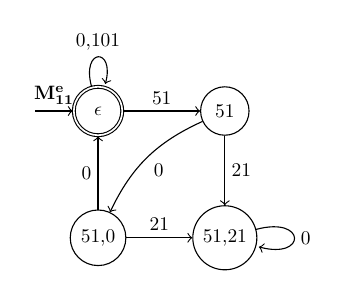
\begin{tikzpicture}
    \node[state,accepting] (1) {$\epsilon$};
    \draw[<-] (1) -- node[above] {$\mathbf{M_{11}^e}$} ++(-.8cm,0);
    \node[state] (2) [right of=1] {51};
    \node[state] (3) [below of=1] {51,0};
    \node[state] (4) [below of=2] {51,21};
    \path
    (1) edge [loop above] node {0,101} (1)
    (1) edge node {51} (2)
    (2) edge [bend right=20] node {0} (3)
    (2) edge node {21} (4)
    (3) edge node {0} (1)
    (3) edge node {21} (4)
    (4) edge [loop right] node {0} (4)
    ;
\end{tikzpicture}
 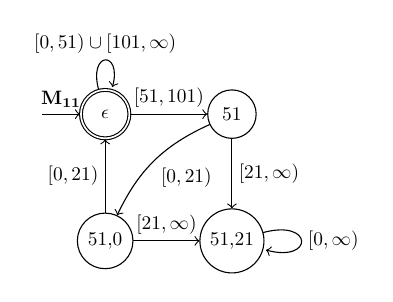
\begin{tikzpicture}
    \node[state,accepting] (1) {$\epsilon$};
    \draw[<-] (1) -- node[above] {$\mathbf{M_{11}}$} ++(-.8cm,0);
    \node[state] (2) [right of=1] {51};
    \node[state] (3) [below of=1] {51,0};
    \node[state] (4) [below of=2] {51,21};
    \path
    (1) edge [loop above] node {$[0,51) \cup [101,\infty)$} (1)
    (1) edge node {$[51,101)$} (2)
    (2) edge [bend right=20] node {$[0,21)$} (3)
    (2) edge node {$[21,\infty)$} (4)
    (3) edge node {$[0,21)$} (1)
    (3) edge node {$[21,\infty)$} (4)
    (4) edge [loop right] node {$[0,\infty)$} (4)
    ;
\end{tikzpicture}

    \end{tabular}
    \caption{An example run of the \alg\ algorithm.}
    \label{fig:example}
\end{figure}


\subsection{Worked Example}\label{subsec:ex}
Suppose we invoke \alg\ to learn the automaton
over non-negative integers that accepts
all words \emph{except} those that
contain a number between 51 and 100 that
is not immediately followed by two numbers
between 0 and 20.

The Boolean algebra we use is the union
of left-closed right-open intervals.
We fix a partitioning function $P$ that assumes
that if $a \in \ell$, $b \in \ell'$,
and there are no $c$ in the input sets
such that $a < c < b$, then the whole
interval $[a,b)$ behaves equivalently to $a$.
For example,
$P(\{0\},\{10\}) = [0,10), [10,\infty)$
and
$P(\{0,20\},\{10\}) = [0,10)\cup[20,\infty), [10,\infty)$.

The trace of the algorithm is illustrated
in Figure~\ref{fig:example}.
\alg\ begins by initializing an observation table
so that $S = \{\epsilon\}$, $R = \{0\}$
(the 0 is an arbitrary character from $\Sigma$
and is used purely so that the table contains
$\epsilon \cdot a$ for some $a$),
and $E = \{\epsilon\}$.
The appropriate membership queries are
made to the oracle, resulting in the table $\mathbf{T_1}$.
$\mathbf{T_1}$ is cohesive, so it is used to construct the evidence automaton
$\mathbf{M_1^e}$, and by calling the partitioning function
$P$ on the outgoing transitions of each state in $\mathbf{M_1^e}$---in
this case just $P(\{0\}) = [0,\infty)$---the
\SFA\ $\mathbf{M_1}$ is conjectured.
The oracle is given $\mathbf{M_1}$ as an equivalence query,
and it returns the single-character word 51
as a counterexample.
51 is added to $R$ in the observation table,
as would all of its prefixes if it were a word of length
greater than one,
and a membership query is asked for $51\cdot\epsilon$,
resulting in table $\mathbf{T_2}$.

$\mathbf{T_2}$ is not closed, since $\textit{row}(51) = -$
and there is no $s \in S$ with $\textit{row}(s) = -$.
Accordingly, 51 represents a path to a new state,
so it is moved from $S$ to $R$, and a continuation
$51,0$ is added to $R$.  This produces
table $\mathbf{T_3}$, which is now cohesive
and thus admits the construction
of the evidence automaton $\mathbf{M_3^e}$
and ultimately the \SFA\ $\mathbf{M_3}$
through the use of the partitioning function:
for example, for the outgoing transitions of the initial state,
$P(\{0\},\{51\}) = [0,51), [51,\infty)$.
An equivalence query sent to the oracle
returns the counterexample of 101.

Adding 101 to $R$ results in the
cohesive table $\mathbf{T_4}$ and the \SFA\ $\mathbf{M_4}$,
and the oracle provides the counterexample $51,0,0$.
$51,0,0$ is added to $R$ (all of its prefixes
are already present in $S \cup R$),
resulting in the table $\mathbf{T_5}$ which is not
consistent:
observe that $\textit{row}(51) = - = \textit{row}(51,0)$,
but $\textit{row}(51\cdot0) = - \neq + = \textit{row}(51,0\cdot0)$.
This means that $51$ and $51,0$ actually lead
to different states, which will be addressed in two stages.
First, following the rule \emph{make-consistent}, since
$f(51\cdot0\cdot\epsilon) \neq f(51,0\cdot0\cdot\epsilon)$,
we add $0\cdot\epsilon$ to $E$ to distinguish
the states led to by $51$ and $51,0$,
which produces table $\mathbf{T_6}$.
Applying \emph{close} to $\mathbf{T_6}$ results in $\mathbf{T_7}$,
which is then cohesive
(we added an element to $E$, which would
normally require applying \emph{evidence-close},
but it happens to be that $\mathbf{T_7}$ is already
evidence-closed) and produces
an \SFA\ $\mathbf{M_7}$.
The counterexample $51,21,0$
requires adding it as well as the prefix $51,21$
to $R$, producing table $\mathbf{T_8}$.

$\mathbf{T_8}$ is also inconsistent,
since $\textit{row}(51) = -,- = \textit{row}(51,21)$
but $\textit{row}(51\cdot0) = -,+ \neq -,- = \textit{row}(51,21\cdot0)$.
Since $f(51\cdot0\cdot0) \neq f(51,21\cdot0\cdot0)$,
we add $0\cdot0$ to $E$
to distinguish $51$ from $51,21$,
and evidence-close the table to get $\mathbf{T_9}$.
Closing and evidence-closing this table results in $\mathbf{T_{10}}$,
the conjecture $\mathbf{M_{10}}$, the counterexample
$51,0,21$, the table $\mathbf{T_{11}}$, and finally
the automaton $\mathbf{M_{11}}$ which passes
the equivalence query.

\section{Learnability and its Properties}
\label{sec:learnability}

Whether an \SFA can be learned and, if so, the complexity of learning that \SFA,
depends on a more fundamental property concerning the \emph{learnability}
of the underlying Boolean algebra.
In \alg,
this notion of learnability determines the
complexity of the algorithm.
We first provide a definition for an algebra's learnability
with respect to the inputs given to a partitioning function
and then connect these inputs to the queries given to the oracle
during the learning algorithm.

\subsection{Learnability of a Boolean Algebra}

Fix a partitioning function $P$ over a Boolean algebra $\mathcal{A}$.
Let $C$ denote a concept class for which each concept $c \in C$ is a finite partition
of $\mathfrak{D}_\mathcal{A}$ using predicates in $\Psi_\mathcal{A}$,
and let $G$ denote the set of \emph{generators} which, informally,
provide a sequence of counterexamples---elements
in $\mathfrak{D}_\mathcal{A}$---to update the sets given to $P$.
We analyze how many times a generator $g$ must make an update
before $P$ learns a desired partition.
A generator $g \in G$ can be thought of as a function
that takes as input
a tuple $(L, c_\text{guess}, c_\text{target})$---where
$L$ is the list of subsets of $\mathfrak{D}_\mathcal{A}$
given as input to $P$,
$c_\text{guess} \in C$ is a partition of $\mathfrak{D}_\mathcal{A}$
consistent with $L$, and
$c_\text{target} \in C$ is the target partition---and
outputs a new list $L'$ of $\mathfrak{D}_\mathcal{A}$-subsets.
We say $g$ provides sets to $P$ to refer to
the iterative process in which
$L_0 = \lbrack \emptyset \rbrack$ and
$L_{i+1} = g(L_i, P(L_i), c_\text{target})$.
Intuitively, a generator iteratively updates a list of sets
to be given to a partitioning function so that
the output of that function approaches the target partition.

Additionally, the generators are subject to the following restrictions
that ensure a sense of monotonicity:
%
\rone the output $L'$ is \emph{greater than}
the input $L$ in the sense that 
$\forall a \in \mathfrak{D}_\mathcal{A}
\lbrack (\exists \ell \in L \ldotp a \in \ell) \rightarrow
(\exists \ell' \in L' \ldotp a \in \ell')\rbrack$
(a character present in the input
will always be present in future iterations);
\rtwo if $a_1 \in \ell_i \in L$ and $a_2 \in \ell_j \in L$
and $i \neq j$, then
it cannot be that there is some $\ell' \in L'$ and
both $a_1 \in \ell'$ and $a_2 \in \ell'$
(if the generator says two elements belong to different
sets in a partition, that must be true for all future iterations);
and \rthree either
the number of sets in $L'$ is larger than
the number of sets in $L$, or
at least one $a \in \mathfrak{D}_\mathcal{A}$
that was not present in any $\ell \in L$ is present in some $\ell' \in L'$
%
Also, the inputs to the generator are subject to a notion of consistency:
if $a_1 \in \ell_i \in L$ and $a_2 \in \ell_j \in L$
such that $i \neq j$, then there is no
$\varphi \in c_\text{target}$ such that
$\{a_1, a_2\} \subseteq \den{\varphi}$.

This definition of a generator exactly captures
the high-level process of updating the observation
table in our algorithm via queries to the oracle
and \emph{projecting} those changes onto
the individual lists of sets that are given
to the partitioning function for the creation
of the conjectured \SFA.
For example, in Figure~\ref{fig:example},
the evidence for the outgoing transitions
of the $\epsilon$-state is provided by a generator such that
$L_1 = \lbrack\{0\}\rbrack$,
$L_2 = \lbrack\{0\}, \{51\}\rbrack$,
and $L_3 = \lbrack\{0,101\},\{51\}\rbrack$.
Below we will formalize
a notion of learnability with respect
to these generators, and it will thus
bear a close correspondence to the
complexity of learning an \SFA.

\begin{definition}[$s_g$-learnability]
    Given a Boolean algebra $\mathcal{A}$,
    a partitioning function $P$, and
    a generator $g \in G$,
    we say the pair $(\mathcal{A}, P)$ is \emph{$s_g$-learnable}
    if there exists an implicit function
    $s_g : C \rightarrow \mathbb{N}$
    such that $P$ needs as input a list of sets,
    provided by $g$,
    with total size at most $s_g(c)$
    to discover a target partition $c \in C$.
    Furthermore, we say $\mathcal{A}$ itself
    is $s_g$-learnable if there exists
    a partitioning function $P$
    such that $(\mathcal{A}, P)$ is $s_g$-learnable.
\end{definition}

We also classify $\mathcal{A}$
as belonging to a \emph{learning class}
that depends on these $s_g$ functions---but
first we need an auxiliary notion of the \emph{size}
of a partition.

\begin{definition}[DNF-Size of a partition]
    Let $C$ be the set of partitions of $\mathcal{A}$.
    Each $c \in C$ is a list $\varphi_1, \ldots, \varphi_n$:
    we can expand each $\varphi_i$ to a minimal
    disjunctive-normal-form formula $\bigvee_j \psi_{i,j}$
    such that
    $c' = \psi_{1,1}, \ldots, \psi_{1,m_1}, \ldots, \psi_{n,1}, \ldots, \psi_{n,m_n}$
    is a partition of $\mathcal{A}$ that is
    at least as fine as $c$.
    We say the \emph{DNF-size} of $c$
    is the length of the list of such a minimal $c'$.
\end{definition}

\begin{example}
    The partition $\{x < 5 \lor x > 10, 5 \leq x \land x \leq 10\}$
    has DNF-size 3.
\end{example}

\begin{definition}[Learning Class]
    For a fixed Boolean algebra $\mathcal{A}$
    if there exists a $g \in G$ such that
    $\mathcal{A}$ is $s_g$-learnable, then
    \begin{itemize}
        \item if $s_g$ is a constant function,
            i.e. $\exists k \forall c \ldotp s_g(c) = k$,
            we say $\mathcal{A} \in \mathcal{C}_\textit{const}^\exists$
        \item if $s_g$ is a function only of the DNF-size of $c$,
            we say $\mathcal{A} \in \mathcal{C}_\textit{size}^\exists$
        \item if $s_g$ is otherwise unconstrained,
            we say $\mathcal{A} \in \mathcal{C}_\textit{finite}^\exists$
    \end{itemize}

    Additionally, for some fixed partitioning function $P$,
    if for all $g \in G$,
    $(\mathcal{A}, P)$ is $s_g$-learnable, then
    \begin{itemize}
        \item if each $s_g$ is a constant function,
            we say $\mathcal{A} \in \mathcal{C}_\textit{const}^\forall$
        \item if each $s_g$ is a function only of the DNF-size of $c$,
            we say $\mathcal{A} \in \mathcal{C}_\textit{size}^\forall$
        \item if each $s_g$ is otherwise unconstrained,
            we say $\mathcal{A} \in \mathcal{C}_\textit{finite}^\forall$
    \end{itemize}
\end{definition}
%

\begin{wrapfigure}{r}{0.35\textwidth}
\vspace{-4mm}
\centering
\begin{tabular}{l l l l l}
    $\mathcal{C}_\textit{const}^\forall$ & $\subseteq$~ & $\mathcal{C}_\textit{size}^\forall$ & $\subseteq$~ & $\mathcal{C}_\textit{finite}^\forall$ \\
    ~\rotatebox[origin=c]{-90}{$\subseteq$} & & ~\rotatebox[origin=c]{-90}{$\subseteq$} & & ~\rotatebox[origin=c]{-90}{$\subseteq$} \\
    $\mathcal{C}_\textit{const}^\exists$ & $\subseteq$~ & $\mathcal{C}_\textit{size}^\exists$ & $\subseteq$~ & $\mathcal{C}_\textit{finite}^\exists$ \\
\end{tabular}
\caption{Learning classes. \label{fig:relation}}
\vspace{-5mm}
\end{wrapfigure}
Observe that learning classes are partially-ordered by the subset relation
shown in Figure~\ref{fig:relation}.
This categorization is convenient for reasoning about
different instantiations of domains and oracles.
For example:
%
\rone When $\mathcal{A} \in \mathcal{C}_\textit{const}^\forall$, learning a
partition over $\mathfrak{D}_\mathcal{A}$ is equivalent
to the machine-learning notion of a mistake-bound~\cite{littlestone88}.
%
\rtwo The equality algebra for any finite alphabet is in $\mathcal{C}_\textit{const}^\forall$.
%
\rthree The interval algebra over the integers or rationals
is in $\mathcal{C}_\textit{size}^\exists$;
if the oracle provides lexicographically minimal counterexamples,
the number of times the partitions must be updated
through the generator is determined by the number of
connected regions in the partition,
as illustrated in~\cite{mens15}
and as applicable for Figure~\ref{fig:example}.
%
The integer case is also in $\mathcal{C}_\textit{finite}^\forall$,
since after arbitrary counterexamples are found beyond the least
and greatest finite bounds in the partition, $m$ and $M$ respectively,
at most $M - m$ more counterexamples are required.
%
\rfour Using enumeration, linear rational arithmetic is in $\mathcal{C}_\textit{finite}^\forall$.
%


Since for each state in an \SFA, the set of outgoing transitions
forms a partition of the alphabet, i.e. a concept in $C$,
the number of counterexamples
needed to learn the entire automaton is related to
the sum of $s_g(c)$ for each state's outgoing transitions.
Hence, the complexity of learning depends on
\rone the choice of the partitioning function and, potentially,
\rtwo the quality of counterexamples provided by the oracle.

\begin{theorem}[SFA Learnability]\label{thm:learn}
    If $M$ is an \SFA over a learnable Boolean algebra $\mathcal{A}$ with $n$ states,
    then the number of equivalence queries
    needed to learn $M$ is bounded above by $n^2 \sum_{q_i \in Q} s_{g_i}(c_i)$,
    where $s_{g_i}$ is the projection of the oracle
    onto learning the partition $c_i$
    for the outgoing transitions of state $q_i$.
\end{theorem}

The notion of an algebra's learning class can have powerful ramifications
in conjuction with the result of Theorem~\ref{thm:learn}.
For example, if an \SFA uses a Boolean algebra contained
in $\mathcal{C}_\textit{finite}^\forall$, then the use
of the appropriate partitioning function guarantees termination
of the learning algorithm, independent of the quality of counterexamples
produced from equivalence queries.
%The automaton $\mathbf{M_{11}}$ from Figure~\ref{fig:example}
%learned with the partitioning function from Section~\ref{subsec:ex}
%and an oracle that provides minimal counterexamples instantitates
%$\mathcal{C}_\textit{size}^\exists$, and for this automaton
%$n = 4$ and $\sum_i s_{g_i}(c_i) = 8$; consequently,
%the number of equivalence queries utilized by the algorithm
%is pessimistically bounded from above by 128.
%%%%the bound is potentially taken from the max, not the sum
Investigating which of the subset relations in Figure~\ref{fig:relation}
are strict subsets, as well as what (if any) algebras fall outside
of $\mathcal{C}_\textit{finite}^\exists$ are interesting
future problems.

\subsection{Composing Learnable Algebras}\label{sec:comp}

The definition of learnability described prior has
the remarkable property that it is preserved by some 
constructions that combine Boolean algebras,
such as the \emph{disjoint union} and the \emph{cartesian product}.
In these cases, a partitioning function for the 
resultant algebra can be constructed by using partitioning
functions for the original algebras as black boxes;
This allows us to phrase
the learnability of the constructed algebra
in terms of the learnability of the individual algebras.

\begin{definition}[Disjoint Union Algebra]
    Let $\mathcal{A}_1, \mathcal{A}_2$ be boolean algebras.
    Their \emph{disjoint union algebra}
    $\mathcal{A}_\uplus = (\mathfrak{D}, \Psi, \den{\_}, \bot, \top, \vee, \wedge, \neg)$,
    which we denote $\mathcal{A}_\uplus = \mathcal{A}_1 \uplus \mathcal{A}_2$,
    is constructed as follows:\footnote{In our definition, we use
    $\mathfrak{D}_{\mathcal{A}_1} \uplus \mathfrak{D}_{\mathcal{A}_2}$
    to denote the disjoint union of sets; rigorously, 
    when the sets are not already disjoint,
    this is constructed by taking
    $(\mathfrak{D}_{\mathcal{A}_1} \times \{1\}) \cup
    (\mathfrak{D}_{\mathcal{A}_2} \times \{2\})$ and lifting
    all the remaining constructs appropriately.}
    $$
    \begin{array}{c}
        \mathfrak{D} = \mathfrak{D}_{\mathcal{A}_1} \uplus \mathfrak{D}_{\mathcal{A}_2} \qquad
        \Psi = \Psi_{\mathcal{A}_1} \times \Psi_{\mathcal{A}_2} \qquad
        \den{(\varphi_{\mathcal{A}_1}, \varphi_{\mathcal{A}_2})} = 
            \den{\varphi_{\mathcal{A}_1}}_{\mathcal{A}_1} \uplus
            \den{\varphi_{\mathcal{A}_2}}_{\mathcal{A}_2} \\
        \bot = (\bot_{\mathcal{A}_1}, \bot_{\mathcal{A}_2}) \qquad
        \top = (\top_{\mathcal{A}_1}, \top_{\mathcal{A}_2}) \qquad
        \neg (\varphi_{\mathcal{A}_1}, \varphi_{\mathcal{A}_2}) =
            (\neg_{\mathcal{A}_1} \varphi_{\mathcal{A}_1},
            \neg_{\mathcal{A}_2} \varphi_{\mathcal{A}_2})\\
        (\varphi_{\mathcal{A}_1}, \varphi_{\mathcal{A}_2}) \vee
            (\varphi_{\mathcal{A}_1}', \varphi_{\mathcal{A}_2}') = 
            ((\varphi_{\mathcal{A}_1} \vee_{\mathcal{A}_1} \varphi_{\mathcal{A}_1}'),
            (\varphi_{\mathcal{A}_2} \vee_{\mathcal{A}_2} \varphi_{\mathcal{A}_2}')) \\
        (\varphi_{\mathcal{A}_1}, \varphi_{\mathcal{A}_2}) \wedge
            (\varphi_{\mathcal{A}_1}', \varphi_{\mathcal{A}_2}') = 
            ((\varphi_{\mathcal{A}_1} \wedge_{\mathcal{A}_1} \varphi_{\mathcal{A}_1}'),
            (\varphi_{\mathcal{A}_2} \wedge_{\mathcal{A}_2} \varphi_{\mathcal{A}_2}')) \\        
    \end{array}
    $$
\end{definition}

If $\mathcal{A}_1$ has partitioning function $P_1$
and $\mathcal{A}_2$ has partitioning function $P_2$,
then we can construct a partitioning function $P_\uplus$
for $\mathcal{A}_\uplus = \mathcal{A}_1 \uplus \mathcal{A}_2$:
$P_\uplus$ takes as input a list $L_\uplus$ of sets
where each set $\ell_{\uplus_i} \subset \mathfrak{D}_{\mathcal{A}_1} \uplus \mathfrak{D}_{\mathcal{A}_2}$.
We decompose $L_\uplus$ into $L_{\mathfrak{D}_1}$ and $L_{\mathfrak{D}_2}$, two lists of sets
of $\ell_{1_i} \subset \mathfrak{D}_{\mathcal{A}_1}$
and $\ell_{2_i} \subset \mathfrak{D}_{\mathcal{A}_2}$, respectively:
for each $a \in \ell_{\uplus_i}$, 
if $a \in \mathfrak{D}_{\mathcal{A}_1}$, then we add $a$ to $\ell_{1_i}$, and otherwise
if $a \in \mathfrak{D}_{\mathcal{A}_2}$, then we add $a$ to $\ell_{2_i}$.
We obtain $L_{\Psi_1} = P_1(L_{\mathfrak{D}_1})$
and $L_{\Psi_2} = P_2(L_{\mathfrak{D}_2})$.
We construct $L_{\Psi_\uplus}$ by taking
$\varphi_{\uplus_i} = (\varphi_{1_i}, \varphi_{2_i})$ for all $i$,
return $L_{\Psi_\uplus}$, and terminate.

The disjoint union is useful since, for example,
we can represent arbitrary intervals over the integers
as the disjoint union of \rone intervals over non-negative integers
and \rtwo intervals over negative integers.
In other words, a partitioning function suited
for a single notion of $\infty$ can be extended
to capture two.

\begin{theorem}[Disjoint Union Algebra Learnability]\label{thm:du}
    Given Boolean algebras $\mathcal{A}_1, \mathcal{A}_2$
    with partitioning functions $P_1, P_2$,
    $(\mathcal{A}_1, P_1)$ is $s_{g_1}$-learnable
    and $(\mathcal{A}_2, P_2)$ is $s_{g_2}$-learnable
    if and only if there exists $g_\uplus$ such that their disjoint union algebra
    $(\mathcal{A}_\uplus, P_\uplus)$ is $s_{g_\uplus}$-learnable,
    where $s_{g_\uplus}(c) = s_{g_1}(c_1) + s_{g_2}(c_2)$
    and $c_1$ and $c_2$ are the restrictions of $c$
    to $\mathfrak{D}_{\mathcal{A}_1}$ and $\mathfrak{D}_{\mathcal{A}_2}$,
    respectively.
\end{theorem}

\begin{corollary}\label{thm:ducor}
    If $\mathcal{A}_1$
    and $\mathcal{A}_2$ are in learning class $\mathcal{C}$,
    then their disjoint union $\mathcal{A}_\uplus$ is also in learning class
    $\mathcal{C}$.
\end{corollary}

We present a similar construction for the \emph{product}
of two Boolean algebras.

\begin{definition}[Product Algebra]
    Let $\mathcal{A}_1, \mathcal{A}_2$ be boolean algebras.
    Their \emph{product algebra}
    $\mathcal{A}_\times = (\mathfrak{D}, \Psi, \den{\_}, \bot, \top, \vee, \wedge, \neg)$,
    which we denote $\mathcal{A}_\times = \mathcal{A}_1 \times \mathcal{A}_2$,
    is constructed as follows:
    $$\begin{array}{c}
        \mathfrak{D} = \mathfrak{D}_{\mathcal{A}_1} \times \mathfrak{D}_{\mathcal{A}_2} \quad
        \Psi = 2^{\Psi_{\mathcal{A}_1} \times \Psi_{\mathcal{A}_2}} \quad
        \den{\{(\varphi_{\mathcal{A}_1i}, \varphi_{\mathcal{A}_2i})\}_i} = 
            \textstyle\bigcup_i ~\den{\varphi_{\mathcal{A}_1i}}_{\mathcal{A}_1}
            \times \den{\varphi_{\mathcal{A}_2i}}_{\mathcal{A}_2} \\
        \bot = \{(\bot_{\mathcal{A}_1}, \bot_{\mathcal{A}_2})\} \qquad
        \top = \{(\top_{\mathcal{A}_1}, \bot_{\mathcal{A}_2})\} \\
        \neg\{(\varphi_{\mathcal{A}_1i}, \varphi_{\mathcal{A}_2i})\}_i =
            \textstyle\bigwedge_i\{(\neg_{\mathcal{A}_1} \varphi_{\mathcal{A}_1i}, \top_{\mathcal{A}_2}),
            (\top_{\mathcal{A}_1}, \neg_{\mathcal{A}_2} \varphi_{\mathcal{A}_2i})\}\\        
        \{(\varphi_{\mathcal{A}_1i}, \varphi_{\mathcal{A}_2i})\}_i \vee
            \{(\varphi_{\mathcal{A}_1j}', \varphi_{\mathcal{A}_2j}')\}_j = 
            \{(\varphi_{\mathcal{A}_1i}, \varphi_{\mathcal{A}_2i})\}_i \cup
            \{(\varphi_{\mathcal{A}_1j}', \varphi_{\mathcal{A}_2j}')\}_j \\ 
        \{(\varphi_{\mathcal{A}_1i}, \varphi_{\mathcal{A}_2i})\}_i \wedge
            \{(\varphi_{\mathcal{A}_1j}', \varphi_{\mathcal{A}_2j}')\}_j = 
            \{(\varphi_{\mathcal{A}_1i} \wedge_{\mathcal{A}_1} \varphi_{\mathcal{A}_1j}',
            \varphi_{\mathcal{A}_2i} \wedge_{\mathcal{A}_2} \varphi_{\mathcal{A}_2j}')
            \mid \forall i,j\} \\
    \end{array}$$
\end{definition}

If $\mathcal{A}_1$ has partitioning function $P_1$
and $\mathcal{A}_2$ has partitioning function $P_2$,
then we can construct a partitioning function $P_\times$
for $\mathcal{A}_\times = \mathcal{A}_1 \times \mathcal{A}_2$:
$P_\times$ takes as input a list $L_\times$ of sets
where each set $\ell_{\times_i} \subset \mathfrak{D}_{\mathcal{A}_1} \times \mathfrak{D}_{\mathcal{A}_2}$.
%
We first take the set $D_1 = \{d_1 \mid (d_1, d_2) \in \ell_{\times_i}
\text{ for some } \ell_{\times_i} \in L_\times \}$,
turn it into a list $D_1' = \{d_{1,1}\},\ldots,\{d_{1,n}\}$,
and compute a partition $L_1 = P_1(D_1')$.
Then for each $d_i \in D_1$, we construct a list
$D_{2,d_i}$ where the $j$-th element is the set
$\{d_2 \mid (d_i, d_2) \in \ell_{\times_j}\}$
and compute a partition $L_{2,d_i} = P_2(D_{2,d_i})$.
%
Finally, we initialize the list of predicates to be returned
$L_{\Psi_\times} = \varphi_{\times_1}, \ldots, \varphi_{\times_k}$
so that initially each $\varphi_{\times_i} = \bot$.
Then for all $i$ and each $(d_1, d_2) \in \ell_{\times_i}$,
let $\varphi_{d_1}$ be the predicate in $L_1$ corresponding to
$\{d_1\}$ in $D_1'$
and let $\varphi_{d_2}$ be the predicate in $L_{2,d_1}$
corresponding to the set of $D_{2,d_1}$ that contains $d_2$;
update $\varphi_{\times_i} \gets \varphi_{\times_i} \vee (\varphi_{d_1}, \varphi_{d_2})$.
%
Return $L_{\Psi_\times}$ and terminate.

\begin{example}
    Suppose we want to find a partition over $(x,y) \in \mathbb{Z} \times \mathbb{Z}$
    where each component uses the interval algebra,
    and suppose the input sets are
    $L_\times = [\{(0, 0), (1, 0), (1,2)\}, \{(0,2)\}]$.
    Then $D_1' = [\{0\}, \{1\}]$
    and perhaps $L_1 = P_1(D_1') = [x \leq 0, x > 0]$.
    Then we have
    $D_{2,0} = [\{0\}, \{2\}]$ and
    $D_{2,1} = [\{0,2\}, \emptyset]$.
    Perhaps
    $L_{2,0} = P_2(D_{2,0}) = [y \leq 1, y > 1]$ and
    $L_{2,1} = P_2(D_{2,1}) = [\top, \bot]$.
    Then (without simplification)
    $L_{\Psi_\times} = [(x \leq 0, y \leq 1) \vee (x > 0, \top) \vee (x > 0, \top), (x \leq 0, y > 1)]$
\end{example}

\begin{theorem}[Product Algebra Learnability]\label{thm:prod}
    Given Boolean algebras $\mathcal{A}_1, \mathcal{A}_2$
    with partitioning functions $P_1, P_2$
    and their product algebra $\mathcal{A}_\times$
    with the composite partitioning function $P_\times$,
    let $c \in C_\times$ be the target partition over the product algebra,
    let $c_1 \in C_1$ be the minterms of the $\mathcal{A}_1$-components of $c$, and
    let $c_2 \in C_2$ be the minterms of the $\mathcal{A}_2$-components of $c$.
    \rone If $(\mathcal{A}_1, P_1)$ is $s_{g_1}$-learnable
    and $(\mathcal{A}_2, P_2)$ is $s_{g_2}$-learnable,
    then there exists $g_\times$ such that
    $(\mathcal{A}_\times, P_\times)$ is $s_{g_\times}$-learnable
    where $s_{g_\times}(c) = s_{g_1}(c_1) s_{g_2}(c_2)$.
    \rtwo If $(\mathcal{A}_\times, P_\times)$ is $s_{g_\times}$-learnable,
    then there exist $g_1, g_2$ such that
    $(\mathcal{A}_1, P_1)$ is $s_{g_1}$-learnable
    and $(\mathcal{A}_2, P_2)$ is $s_{g_2}$-learnable
    where $s_{g_\times}(c) = s_{g_1}(c_1) = s_{g_2}(c_2)$.
\end{theorem}

\begin{corollary}\label{thm:prodcor}
    If $\mathcal{A}_1$
    and $\mathcal{A}_2$ are in learning class $\mathcal{C}$,
    then their product $\mathcal{A}_\times$ is also in learning class
    $\mathcal{C}$.
\end{corollary}
Since learnability is closed
under disjoint union and product,
symbolic automata over non-recursive data types can 
be learned using partitioning functions for the component types,
as opposed to necessitating specialized partitioning functions.


\section{Implementation}
\label{sec:implementation}

We implemented \alg in the open-source Java library
Symbolic Automata.
Our modular implementation only requires the programmer to provide
learnable Boolean algebras as input to the learner;
we have already implemented the equality and interval algebras
as well as the disjoint union and product algebras---which
are implemented as meta-algebras and can be instantiated arbitrarily.

We evaluated our algorithm on the examples  presented by
Maler and Mens~\cite{mens15}, who
proposed two extensions of L$^*$
for learning \SFAs where 1) predicates are
union of intervals in $\mathbb{N}$, or
2) predicates are
union of intervals over $\mathbb{N}\times \mathbb{N}$.
Their algorithms  assume that the oracle always provides lexicographically minimal counterexamples,
so that every counterexample identifies a boundary in a partition.
They evaluate their techniques on two automata: one over 
the alphabet $\mathbb{N}$ (Ex. 4.1~\cite{mens15})  and one over the alphabet $\mathbb{N} \times \mathbb{N}$
(Ex. 5.1~\cite{mens15}).

We implemented a partitioning function equivalent to their characterization
of the interval algebra over $\mathbb{N}$.
While, to learn automata over $\mathbb{N} \times \mathbb{N}$,
\cite{mens15} introduces an ad-hoc separate technique that  requires the oracle
to always give locally minimal counterexamples,
in our setting, the algebra for pairs can be trivially implemented as
the Cartesian product of the interval algebra over $\mathbb{N}$ with itself.

We learn the first automaton using 8 equivalence and 23 membership queries,
while their algorithm only requires 7 and 17, respectively.
The former difference is due to their algorithm adding a different suffix
to $E$ than ours, which happens to discover two new states instead of one
and ultimately saves them an equivalence query.
The latter is due to a more refined handling of counterexamples (more in our related work).
Similarly,  we learn the second 
automaton using 28 equivalence and 43 membership queries,
while their algorithm only requires
%We learned this automaton by using the
%meta-partitioning function for product algebras
%presented in Section~\ref{sec:comp},
%which is able to learn the automaton
18 and 20, respectively.
In this case, the discrepancy is amplified because
the algorithm in~\cite{mens15} uses a specialized
implicit partitioning function that avoids the quadratic
blowup caused by the Cartesian product construction
in Theorem~\ref{thm:prod}.
%suggests that using the meta-algebra should
%require about quadratically more
%equivalence queries.
We implemented an analogous specialized partitioning function
directly on the product algebra and were able to learn the same example using
19 equivalence and 30 membership queries.


\section{Related Work}

%Article Aws mentioned~\cite{Nam2006}


%\noindent\textbf{Improvements of L$^*$}
 \alg builds on L$^*$~\cite{angluin87},
for which many extensions have been proposed,
the most advanced one being TTT~\cite{Isberner2014,learnlib}.
%The counterexample processing presented in this paper is simple:
%\emph{every} prefix is added to the observation table.
%Subsequently, new states
%are discovered when the table is not consistent
%and distinguished by naively adding the obvious distinguishing word
%to the set $E$. 
While these extensions could be
applied to \alg  to potentially improve the
size of the observation table, the
number of membership queries is dictated by
the amount of evidence needed for the partitioning function
to generalize.
Our algorithm opens new questions:
Can we efficiently store intermediate predicates computed by the partitioning functions?
Can separating predicates be computed incrementally?

%\textit{Oracle-guided synthesis.}
%Our use of generators is related to the OGIS framework~\cite{JhaS15}, 
%where automata learning 
%its termination are 
% is characterized in terms of the interactions
%with the oracle and the nature of its counterexamples. 
%The OGIS model is too weak for symbolic automata.
%
%Our work more strongly connects the complexity of learning
%with the \emph{learnability} of the underlying algebra,
%which is parametric in the selection of a
%partitioning function.
%The OGIS model focuses on a distinction
%between the expressiveness of infinite-memory and finite-memory
%systems for learning;
%in this paper we assume learning is being done
%only in the context of infinite-memory,
%but we derive stronger results
%about the complexity.
%as opposed to simply whether or not an automaton is learnable.



%Other works on symbolic automata learning,
%for example, binary search the example to find
%an appropriate prefix and suffix such that
%the prefix is added to the states $S$
%and the suffix is added to $E$~\cite{ArgyrosSKK16}.

%\noindent\textbf{Automata Learning and Infinite Alphabets}
Our paper is the first one to provide: 
\rone an algorithm for learning symbolic automata over arbitrary alphabet theories,
with  a notion of learnability that is parametric in both the alphabet theory and the 
oracle (through its projection onto generators), and
\rtwo compositionality properties that permit combining learnable algebras.
We detail our comparison against the most relevant works.


Isberner et al. augment L$^*$ with abstractions to learn automata over 
potentially infinite alphabets~\cite{Isberner2013}.
The algorithm creates abstract symbols to generalize sets of characters,
and the final automaton operates over these abstract symbols. 
Abstractions can cause non-determinism that is resolved using refinement operators.
This approach differs from ours in two aspects. 
First, while the final output of \alg is a symbolic automaton over the target Boolean algebra,
the output in~\cite{Isberner2013} is an automaton operating over a separate abstract alphabet that
is discovered during the learning process and might not necessarily form a Boolean algebra.
Second, our algorithm enjoys well-defined learnability  and compositionality properties over the input Boolean algebras,
while the one in~\cite{Isberner2013} does not provide any such properties.
Maler and Mens~\cite{mens15} instantiate the algorithm proposed in~\cite{Isberner2013} and 
learn automata over the interval algebra
for integers and pair of integers.
%Where we adapt the observation table to
%contain only a subset of what would be included in $L^*$,
%they instead use an observation table whose
%entries are from a \emph{symbolic alphabet},
%or in other words, their table entries
%are elements in $\Psi^*$, each accompanied
%by a \emph{concrete word} in $\Sigma^*$ that
%served as evidence to create the symbolic word.
%This formulation of the observation table is possible
%due to the constraint they make on the oracle:
%it must provide lexicographically minimal counterexamples.
%This way, every counterexample uniquely determines
%the upper or lower bound for a symbolic letter.
%In our technique, which subsumes their method,
%the symbolic alphabet (i.e., the  set of relevant predicates) is dynamically
%generated at each iteration of the algorithm.
As we discussed throughout the paper, 
their results are special cases of our formulation. 
%and,
In fact, their specialized algorithm %for handling pairs of integers \cite{mens15} provides a modified version of the algorithm
for learning automata over pairs of integers
%by constraining that the oracle gives them
%minimal counterexamples in the partial order of the pairs.
%Remarkably, 
is a special case of our Cartesian product of two algebras.
%of the interval algebra with itself.
Using our technique, we can also drop the assumption that the
the oracle provides lexicographically minimal counterexamples,
which simply causes a change  to the $s_g$ functions and learnability.

Argyros et al.~\cite{ArgyrosSKK16} present an algorithm
for learning symbolic automata where
the learnability is parametric with respect
to a \emph{guardgen} method, which
is an equivalent formulation of our partitioning
function.
Their definition of learnability only captures
our learning class $\mathcal{C}_\textit{const}^\forall$ and can therefore only 
describe Boolean algebras operating over finite alphabets or with finitely many predicates.
Our work introduces generators, proposes
a deeper analysis of the learnability of a Boolean algebra,
and shows how learnable algebras can be composed.


The Sigma$^*$ algorithm~\cite{BotincanB13} is a practical algorithm for learning
symbolic transducers, but it does not have learnability guarantees. 
Other algorithms can learn
nominal~\cite{nominal} and register automata~\cite{Cassel2016}. 
In these models, the alphabet is infinite but not structured (i.e., it does not form a Boolean algebra) 
and characters at different positions can be compared using binary relations
(typically equality or simple arithmetic relations).
These models are orthogonal to symbolic automata.

%Learning algorithms have been proposed for nominal automata~\cite{nominal}
%and for a class of extended finite state machines that is related to register automata
%in which the set of relations has been extended to include
%less-than-or-equal as well as equalities over arithmetic expressions
%of the form $y = x + c$~\cite{Cassel2016}.




\noindent\textbf{Acknowledgements}
We would like to thank Alexandra Silva,
Joshua Moerman, and Nimit Singhania
for their feedback on an
early version of this paper.




\bibliographystyle{abbrv}
\bibliography{biblio}

\end{document}
